\documentclass{standalone}

\usepackage{tikz}
\usetikzlibrary{arrows}
\usetikzlibrary{decorations.markings}

\begin{document}

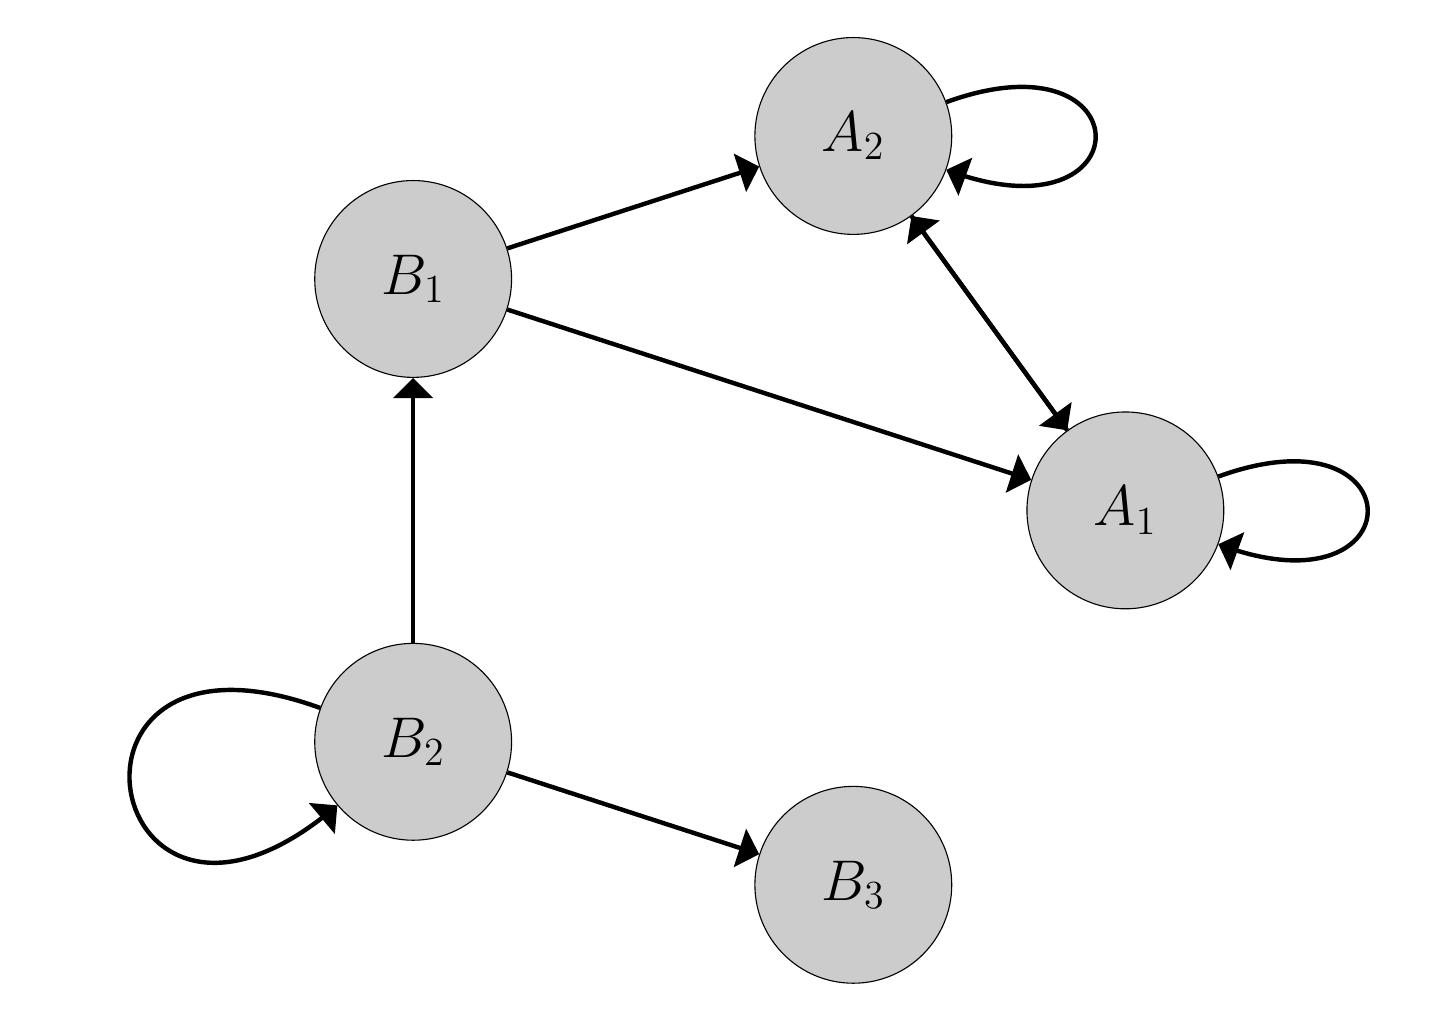
\begin{tikzpicture}
  \node (A1) [style={minimum size=2.5cm,draw=black,fill=black!20!white,text=black,shape=circle}] at (5, 0) {\huge $A_1$};
  \node (A2) [style={minimum size=2.5cm,draw=black,fill=black!20!white,text=black,shape=circle}] at (1.545, 4.755) {\huge $A_2$};
  \node (B1) [style={minimum size=2.5cm,draw=black,fill=black!20!white,text=black,shape=circle}] at (-4.045, 2.939) {\huge $B_1$};
  \node (B2) [style={minimum size=2.5cm,draw=black,fill=black!20!white,text=black,shape=circle}] at (-4.045, -2.939) {\huge $B_2$};
  \node (B3) [style={minimum size=2.5cm,draw=black,fill=black!20!white,text=black,shape=circle}] at (1.545, -4.755) {\huge $B_3$};

  \draw[ultra thick, -triangle 90] (A1) -- (A2);
  \draw[ultra thick, -triangle 90] (A1) to [out=20,in=340,looseness=8] (A1);
  \draw[ultra thick, -triangle 90] (A2) -- (A1);
  \draw[ultra thick, -triangle 90] (A2) to [out=20,in=340,looseness=8] (A2);
  \draw[ultra thick, -triangle 90] (B1) -- (A1);
  \draw[ultra thick, -triangle 90] (B1) -- (A2);
  \draw[ultra thick, -triangle 90] (B2) -- (B1);
  \draw[ultra thick, -triangle 90] (B2) to [out=160,in=220,looseness=8] (B2);
  \draw[ultra thick, -triangle 90] (B2) -- (B3);

\end{tikzpicture}

\end{document}
